\documentclass{report}
\usepackage[
    a4paper,
    top = 2cm,
    left = 2cm,
    bottom = 2cm,
    ]{geometry}
\usepackage{graphicx}
\usepackage{algorithm2e}
\pagestyle{empty}
\newcommand\tab[1][1cm]{\hspace*{#1}}

\title{\Huge Data Structures \\ HW2}
\author{\huge Sina Rostami \\\huge \textbf{9822143}}
\date{Fall 2020}


\begin{document}
    \begin{figure}
        
\includegraphics[height = 30mm,width = 40mm]{../kntu_logo.jpg}
    \end{figure}
    \maketitle
    \section*{Problem 1:}
        \textbf{Pseudo-Code}
        \begin{algorithm}
            let \textit{linked\_list} be the linked-list we want to reverse.\\
            let \textit{size} be the size of the linked\_list.\\
            \For(){i in range(0, size / 2) }{
                let \textit{temp\_node1} points to the head of the linked-list\\
                do \textit{(i)} times:\\
                \tab \textit{temp\_node1} $\gets$ \textit{temp\_node1.next}\\
                let \textit{temp\_node2} points to the head of the linked-list\\
                do \textit{(size - i - 1)} times:\\
                \tab \textit{temp\_node2} $\gets$ \textit{temp\_node2.next}\\
                \textbf{swap} data of \textit{temp\_node1} and \textit{temp\_node2}.
            }
            Now the list have reversed.\\
            you can see the source code of the implementation in the $src$ directory.\\
        \end{algorithm}
    \section*{Problem 2:}
        we can represent the sparce matrix in linked-list representaion.\\
        for that :\\
            1. each Node has 2 more fields as the $i\ and\ j$ index for representing where the data was in the matrix\\ 
            2. each Node has pointers to its right side Node.\\
            3. we use index nodes to represent rows of the matrix in the linked-list\\
        for the given example matrix we have : \\
        \begin{figure}[hbt!]
            \centering
            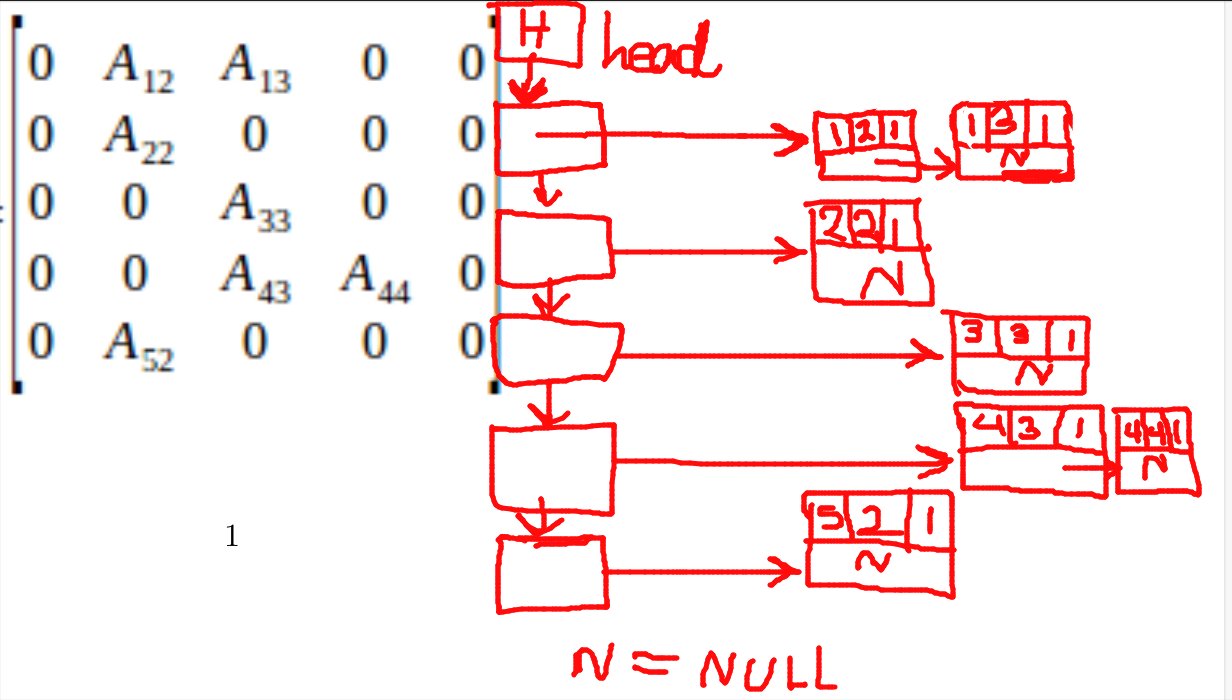
\includegraphics[height = 50mm,width = 120mm]{p2.png}
        \end{figure}
    \section*{Problem 3:}
        we can do this by followings :\\
        1. iterate over array and push them in the stack.\\
        2. now pop the stack (size of array) times and put them in the array.\\
        \textbf{Pseudo-Code}
        \begin{algorithm}
            \For(){i in the array}{
                push i to the stack.
            }
            let index := 0.\\
            \While(){the stack is not empty}{
                let elem := stack.pop\\
                put elem in the index-th cell of the array\\
                index $\gets$ index + 1
            }
        \end{algorithm}
    \section*{Problem 4:}
        \huge A.\\ \normalsize
            popped elements are : [h, s, f]\\
            elements in the stack are : [d, m]\\
        \huge B.\\ \normalsize
            dequeued elements are : [d, h, f]\\
            elements in the queue are : [s, m]\\
    \section*{Problem 5:}
        \huge a) \normalsize 2, 4, 5, 3, 1 \\
        \begin{tabular}{| l | c |}
            \hline
            \Large push (1) &\Large [$\emptyset$]\\
            \hline
            \Large push (2) &\Large [$\emptyset$]\\
            \hline
            \Large pop &\Large [2]\\
            \hline
            \Large push (3) &\Large [2]\\
            \hline
            \Large push (4) &\Large [2]\\
            \hline
            \Large pop &\Large [2, 4]\\
            \hline
            \Large push (5) &\Large [2, 4]\\
            \hline
            \Large pop &\Large [2, 4, 5]\\
            \hline
            \Large pop &\Large [2, 4, 5, 3]\\
            \hline
            \Large pop &\Large [2, 4, 5, 3, 1]\\
            \hline
        \end{tabular}\\
        \huge b) \normalsize 1, 3, 5, 4, 2.\\
        \begin{tabular}{| l | c |}
            \hline
            \Large push (1) &\Large [$\emptyset$]\\
            \hline
            \Large pop &\Large [1]\\
            \hline
            \Large push (2) &\Large [1]\\
            \hline
            \Large push (3) &\Large [1]\\
            \hline
            \Large pop &\Large [1, 3]\\
            \hline
            \Large push (4) &\Large [1, 3]\\
            \hline
            \Large push (5) &\Large [1, 3]\\
            \hline
            \Large pop &\Large [1, 3, 5]\\
            \hline
            \Large pop &\Large [1, 3, 5, 4]\\
            \hline
            \Large pop &\Large [1, 3, 5, 4, 2]\\
            \hline
        \end{tabular}\\
 \\ \\ \\
 \\ \\ \\
 \\ \\ \\
 \\ \\ \\
 \\ \\ \\
    \section*{Problem Bounce:}
        we use $q_1, q_2$ for implementation.\\
    for the Push method abstraction :
        \begin{algorithm}
            \If{$q_1$.isEmpty()}{
                $q_1.enqueue(element)$\\
            }
            \Else(){
                $current\_size := q_1.size()$\\
                \For(){i in (0, $current\_size$)}{
                    $q_2.enqueue(q_1.dequeue())$\\
                }
                $q_1.enqueue(element)$\\
                \For(){i in (0, $current\_size$)}{
                    $q_1.enqueue(q_2.dequeue())$\\
                }
            }
        \end{algorithm}\\
    and for the Pop method abstraction :
        \begin{algorithm}
            \Return{$q_1.dequeue()$}
        \end{algorithm}


\end{document}